% Schema of Labs on a class
% Author: Cristo J. Alanis
\documentclass[11pt]{standalone}
\usepackage{tikz}
\usetikzlibrary{arrows}
% Define the layers to draw the diagram
\pgfdeclarelayer{background}
\pgfdeclarelayer{foreground}
\pgfsetlayers{background,main,foreground}

% Define block styles
\tikzstyle{materia}=[draw, fill=blue!12, text width=6.0em, text centered,
  minimum height=1.5em]
% \tikzstyle{practica} = [materia, text width=8em, minimum width=10em, minimum height=3em, rounded corners,]
\tikzstyle{practica} = [materia,text width = 12em, minimum height=3em, rounded corners]
\tikzstyle{texto} = [above, text width=6em, text centered]
\tikzstyle{linepart} = [draw, thick, color=black!50, -latex', dashed]
\tikzstyle{line} = [draw, thick, color=black!50, -latex']
\tikzstyle{ur}=[draw, text centered, minimum height=0.01em]

% Define distances for bordering
\newcommand{\blockdist}{1.3}
\newcommand{\edgedist}{1.5}

\newcounter{practicaCounter}

\newcommand{\practica}[1]{\stepcounter{practicaCounter} node (p\arabic{practicaCounter}) [practica]
  {#1}}

% Draw background
\newcommand{\background}[5]{%
  \begin{pgfonlayer}{background}
    % Left-top corner of the background rectangle
    \path (#1.west |- #2.north)+(-0.5,0.5) node (a1) {};
    % Right-bottom corner of the background rectanle
    \path (#3.east |- #4.south)+(+0.5,-0.25) node (a2) {};
    % Draw the background
    \path[fill=yellow!20,rounded corners, draw=black!50, dashed]
      (a1) rectangle (a2);
    \path (a1.east |- a1.south)+(0.8,-0.3) node (u1)[texto]
      {\scriptsize\textit{Unidad #5}};
  \end{pgfonlayer}}

\newcommand{\transreceptor}[3]{%
  \path [linepart] (#1.east) -- node [above]
    {\scriptsize Transreceptor #2} (#3);}

\usepackage{bookman}
% \fontfamily{sf}\selectfont

\begin{document}
\sffamily
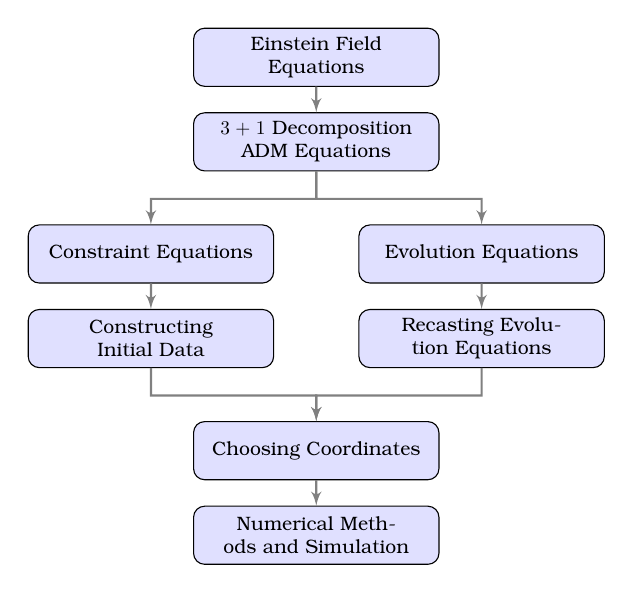
\begin{tikzpicture}[scale=0.7,transform shape]

  % Draw diagram elements
  \path node (p1) [practica] {Einstein Field Equations};

  \path (p1.south)+(0.0,-1.0) node (p2) [practica] {$3+1$ Decomposition \\ ADM Equations};
  \path (p2.south)+(-3.0,-1.5) node (p3) [practica] {Constraint Equations};
  \path (p2.south)+(3.0,-1.5) node (p4) [practica] {Evolution Equations};
  \path (p4.south)+(0.0,-1.0) node (p5) [practica] {Recasting Evolution Equations};
  \path (p3.south)+(0.0,-1.0) node (p6) [practica] {Constructing Initial Data};
  \path (p6.south)+(3.0,-1.5) node (p7) [practica] {Choosing Coordinates};
  \path (p7.south)+(0.0,-1.0) node (p8) [practica] {Numerical Methods and Simulation};

  % \path (p8.east)+(+5.5,0) node (ur1)[ur] {};

  % \path (p7.south)+(0.0,-1.5) node (p9) [practica] {Codificador digital};
  % \path (p8.south)+(0.0,-1.5) node (p10) [practica] {Decodificador digital};
  % \path (p10.east)+(+5.5,0) node (ur2)[ur] {};
  % \path (p9.south)+(0.0,-1.5) node (p11) [practica] {Codificador FDM};
  % \path (p10.south)+(0.0,-1.5) node (p12) [practica] {Decodificador FDM};
  % \path (p12.east)+(+5.5,0) node (ur3)[ur] {};
  % \path (p11.south)+(0.0,-1.5) node (p13) [practica] {Codificador SSTV};
  % \path (p12.south)+(0.0,-1.5) node (p14) [practica] {Decodificador SSTV};
  % \path (p14.east)+(+5.5,0) node (ur4)[ur] {};
  % \path (p14.south)+(-3.0,-1.5) node (p15) [practica] {Conmutaci\'on telef\'onica};
  % \path (p15.south)+(0.0,-1.0) node (p16) [practica] {Telfon\'ia celular an\'aloga};
  % \path (p16.south)+(0.0,-1.5) node (p17) [practica] {Receptor de  telemetr\'ia};
  % \path (p17.south)+(0.0,-1.5) node (p18) [practica] {Gu\'ias de ondas};

  % Draw arrows between elements
  \path [line] (p1.south) -- node [above] {} (p2);

  \path [line] (p2.south) -- +(0.0,-0.5) -- +(-3.0,-0.5)
    -- node [above, midway] {} (p3);
  \path [line] (p2.south) -- +(0.0,-0.5) -- +(3.0,-0.5) -- node [above,midway] {} (p4) ;
  % \path [line] (p3.south) -- node [above] {} (p5) ;

  \path [line] (p3.south) -- node [above] {} (p6);
  \path [line] (p4.south) -- node [above] {} (p5);

  \path [line] (p5.south) -- +(0.0,-0.5) -- +(-3.0,-0.5)
    -- node [above, midway] {} (p7);
  \path [line] (p6.south) -- +(0.0,-0.5) -- +(3.0,-0.5) -- node [above,midway] {} (p7) ;

  \path [line] (p7.south) -- node [above] {} (p8);

  % \path [line] (p2.south) -- +(0.0,-0.5) -- +(+2.5,-0.5)
  %   -- node [above, midway] {} (p4);
  % \path [linepart] (p3.east) -- +(+0.5,-0.0) -- +(+0.5,-1.75)
  %   -- node [left, midway] {} (p4);
  % \path [linepart] (p3.east) -- +(+0.5,-0.0) -- +(+0.5,-1.75)
  %   -- node [left, midway] {} (p4);

  % \path [line] (p4.south) -- +(0.0,-0.5) -- +(-2.5,-0.5)
  %   -- node [above, midway] {} (p6);
  % \path [line] (p5.south) -- +(0.0,-0.5) -- +(+2.5,-0.5)
  %   -- node [above, midway] {} (p6);
  % \path [linepart] (p2.east) -- +(2.75,0.0) -- +(2.75,-5.85)
  %   -- node [right] {} (p6);
  % \path [line] (p6.south) -- +(0.0,-0.25) -- +(-2.5,-0.25)
  %   -- node [above, midway] {} (p7);
  % \path [line] (p6.south) -- +(0.0,-0.25) -- +(+2.5,-0.25)
  %   -- node [above, midway] {} (p8);
  % \path [linepart] (p7.east) -- node [left] {} (p8);
  % \transreceptor{p8}{AM banda 40m}{ur1}

  % \path [line] (p7.south) -- node [above] {} (p9) ;
  % \path [line] (p8.south) -- node [above] {} (p10) ;
  % \path [linepart] (p9.east) -- node [left] {} (p10);
  % \transreceptor{p10}{CW}{ur2}
  % \path [line] (p9.south) -- node [above] {} (p11) ;
  % \path [line] (p10.south) -- node [above] {} (p12) ;
  % \path [linepart] (p11.east) -- node [left] {} (p12);
  % \transreceptor{p12}{FDMDV}{ur3}

  % \path [line] (p11.south) -- node [above] {} (p13) ;
  % \path [line] (p12.south) -- node [above] {} (p14) ;
  % \path [linepart] (p13.east) -- node [left] {} (p14);
  % \transreceptor{p14}{SSTV}{ur4}

  % \path [line] (p14.south) -- +(0.0,-0.5) -- +(-2.5,-0.5)
  %   -- node [above, midway] {} (p15);
  % \path [line] (p13.south) -- +(0.0,-0.5) -- +(+2.5,-0.5)
  %   -- node [above, midway] {} (p15);
  % \path [line] (p15.south) -- node [above] {} (p16) ;
  % \path [line] (p16.south) -- node [above] {} (p17) ;
  % \path [line] (p17.south) -- node [above] {} (p18) ;

  % \background{p3}{p1}{p4}{p2}{I}
  % \background{p3}{p3}{p4}{p5}{II}
  % \background{p3}{p6}{p4}{p7}{III}
  % \background{p3}{p9}{p4}{p10}{IV}
  % \background{p3}{p11}{p4}{p12}{V}
  % \background{p3}{p13}{p4}{p14}{VI}
  % \background{p3}{p15}{p4}{p16}{VII}
  % \background{p3}{p17}{p4}{p17}{VIII}
  % \background{p3}{p18}{p4}{p18}{IX}
\end{tikzpicture}
\end{document}